% Package
\documentclass[11pt]{article}

\usepackage{amsmath}
\usepackage{cite}
\usepackage{graphicx}
\usepackage[utf8]{inputenc}
\usepackage[T1]{fontenc}
\usepackage{lmodern}
\usepackage[ngerman]{babel}
\usepackage{hyphenat}
\usepackage{placeins}

\title{ADP Aufgabe 2 Entwurf, Abgabe 1}
\author{Team 1\\Hugo Protsch, Justin Hoffmann}

% Document
\begin{document}

    \maketitle

    \tableofcontents

    \newpage


    \section{Formales}\label{sec:Formales}

    %! suppress = MissingLabel

    \subsection*{Aufgabenaufteilung}
    Der Entwurf für Insertion Sort wurde zusammen entwickelt.\\
    Der Entwurf für Quick Sort wurde von Hugo Protsch entwickelt.\\
    Der Entwurf für Heap Sort wurde von Justin Hoffmann entwickelt.
    %! suppress = MissingLabel

    \subsection*{Quellenangaben}
    Es wurden lediglich Vorlesungsmaterialien verwendet.
    %! suppress = MissingLabel

    \subsection*{Bearbeitungszeitraum}
    Der gesamte Arbeitsaufwand für den Entwurf belief sich auf ca. 17 Stunden.

    %! suppress = MissingLabel

    \subsection*{Aktueller Stand}
    %! suppress = MissingLabel
    Der Entwurf steht zur Implementation zur Verfugung.

    \subsection*{Änderungen des Entwurfes}
    \begin{itemize}
        \item Quicksort: Pivot-Element Wahl hinzugefügt
        \item
    \end{itemize}


    \section{Insertion Sort}\label{sec:insertion-sort}

    \subsection{Algorithmus}\label{subsec:Ialgorithmus}
    Siehe Abbildung~\ref{fig:insertionS}.
    Bei Insertion Sort wird eine Liste durch das Einfügen von Elementen aus
    einem unsortierten Bereich (zunächst die komplette Liste) in einen sortieren
    Bereich (zunächst leer, <N1>) sortiert.

    Bei dem Einfügen eines Elements E in den sortierten Bereich muss dabei
    jeweils der Bereich bis zu dem Element durchlaufen werden, hinter das das
    Element E eingefügt werden muss (Siehe \frqq Insert into sorted list\flqq
    Subgraph).

    Somit wird der sortierte Bereich mit jeder Iteration um 1 erhöht <E1>.
    Sobald der sortierte Bereich alle Elemente enthält, wird die Liste
    zurückgegeben.
    Bei der Implementation des Algorithmus auf einfach verkettete Listen
    kann der sortierte und unsortierte Bereich getrennt werden.


    \begin{figure}[hbt]
        \caption{Insertion Sort}
        \centering
        \includegraphics[width = 8cm]{insertionS}\label{fig:insertionS}
    \end{figure}
    \FloatBarrier

    \subsection{Laufzeit}\label{subsec:Ilaufzeit}
    Die erwartete Laufzeit beträgt \(O(n^2)\), da bei jeder Iteration das
    einzufügende Element mit allen noch nicht sortierten Elementen verglichen
    wird.
    Im Fall einer bereits sortierten Liste tritt der Best-Case ein.
    Hierbei müssen nur \(n\) Vergleiche durchgeführt werden.
    Somit beträgt die Laufzeit \(\Theta(n)\).

    Bei der Laufzeitmessung überprüfen wir, ob der gemessene Zusammenhang mit
    dem erwarteten übereinstimmt.
    Dafür verwenden wir für den Best-Case zufällige Listen, im Worst-Case
    bereits sortierte Listen.


    \section{Quick Sort}\label{sec:quick-sort}

    \subsection{Algorithmus}\label{subsec:Qalgorithmus}
    Siehe Abbildung~\ref{fig:qsort}.
    Bei Quick Sort wird zunächst willkürlich ein Pivot-Element aus der Liste
    ausgewählt.

    Anschließend wird die Liste in zwei Teile aufgeteilt: Die Liste L erhält
    alle Elemente, die kleiner als das Pivot-Element sind, die Liste R alle
    Elemente, die größer als das Pivot-Element sind.
    Dafür wird die Liste elementweise durchlaufen und jedes Element mit dem
    Pivot-Element verglichen.
    Die Reihenfolge der Elemente in den Listen spielt keine Rolle.
    Das Pivot-Element selber kommt nicht in den Listen vor.

    Da alle Elemente, die kleiner als das Pivot-Element sind und alle Elemente,
    die größer als das Pivot-Element sind nun getrennt vorliegen, ist die
    Position des Pivots eindeutig als 'zwischen den Listen L und R' bestimmt.
    Somit kann der Algorithmus rekursiv auf die jeweiligen Listen erneut
    angewandt werden.

    Das Pivot-Element wird an die Liste R vorangestellt.
    Die Liste L wird der Liste R, inklusive Pivot, vorangestellt.
    Die Liste ist nun sortiert.\\

    \begin{figure}[hbt]
        \caption{Quicksort}
        \centering
        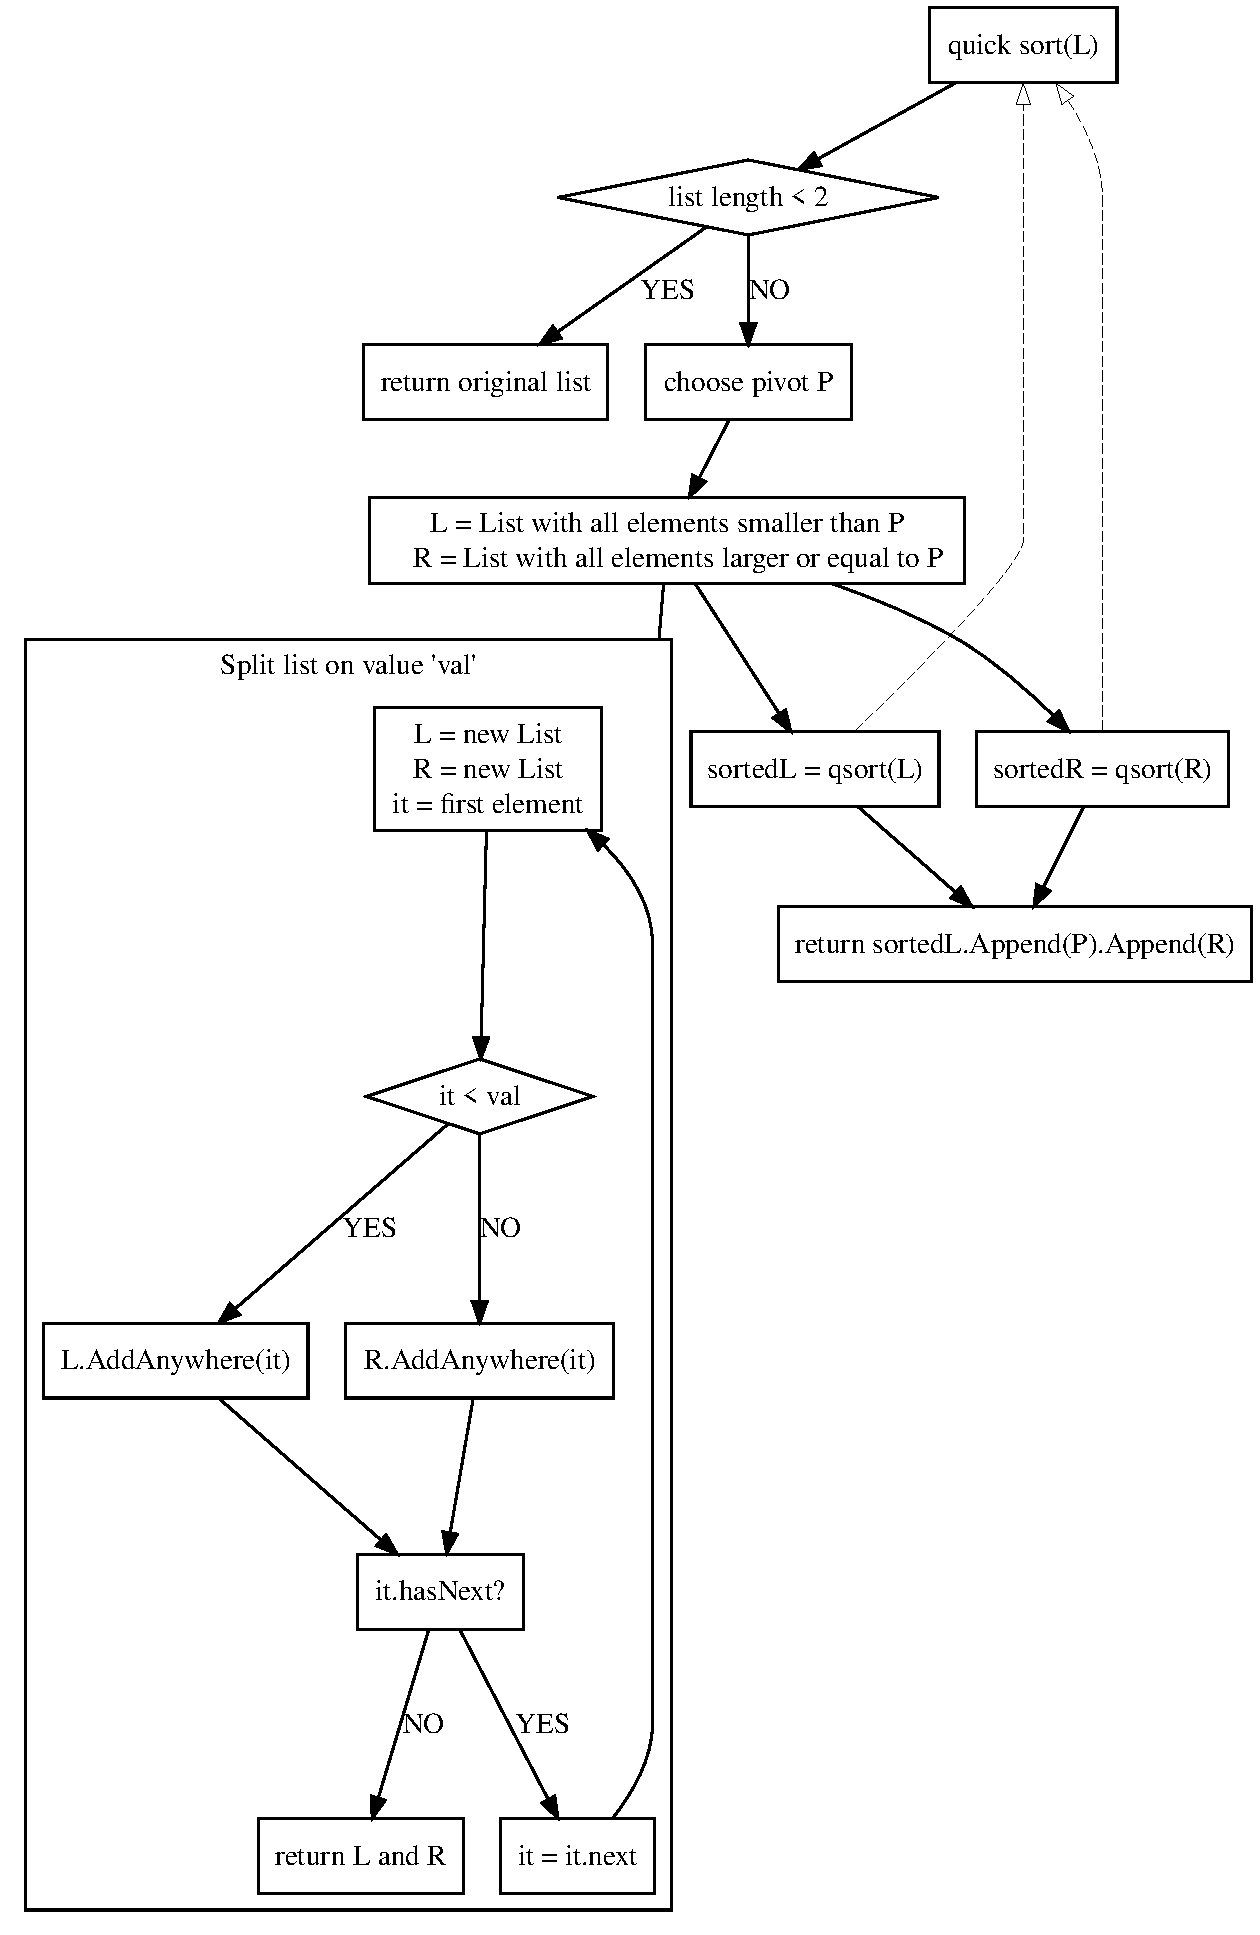
\includegraphics[width = 8cm]{qsort.pdf}\label{fig:qsort}
    \end{figure}

    Für die Wahl des Pivot-Elementes werden insgesamt 5 Methoden implementiert:
    \begin{itemize}
        \item left -- wählt das erste Elemente der Liste
        \item middle -- wählt das mittlere Element der Liste
        \item right -- wählt das letzte Element der Liste
        \item median -- wählt den Median der drei obigen Werte
        \item random -- wählt ein zufällig ausgewähltes Element der Liste
    \end{itemize}

    Des Weiteren soll bei der Implementation des Algorithmus ab einem
    Schwellenwert auf Insertion Sort umgeschaltet werden.
    Dafür wird zu Beginn die Länge der Liste abgefragt, falls diese unter dem
    übergebenem Schwellenwert liegt, wird restliche Liste stattdessen
    mithilfe von Insertion Sort sortiert.

    \FloatBarrier

    \subsection{Laufzeit}\label{subsec:Qlaufzeit}

    Die Laufzeit beträgt im Best-Case \(\Omega (n \cdot \log(n))\), da bei
    gut gewähltem Pivot-Elementen die Anzahl an Vergleichen mit jedem
    Rekursionsschritt halbiert wird, wobei die Teillisten trotzdem durchlaufen
    werden müssen.
    Wenn das Pivot-Element bei jeder Iteration schlecht gewählt ist (kleinstes
    oder größtes Element in der List), beträgt die Laufzeit \(O(n^2)\), da
    jeweils eine Partition die Größe 1 hat und die Anzahl an Vergleichen
    somit nicht reduziert wird.

    Bei der Laufzeitmessung testen wir, ob die Komplexität des implementierten
    Algorithmus mit der erwarteten übereinstimmt.
    Um den Worst-Case zu überprüfen, nutzen wir bereits sortierte Listen und
    wählen das letzte bzw. erste Element als Pivot-Element.
    Für den Best-Case nutzten wir zufällig generierte Listen.\\

    Wir ermitteln des Weiteren die Elementanzahl, ab der Quicksort schneller
    als Insertion Sort ist und wie sich die unterschiedlich Methoden, das
    Pivot-Element auszuwählen, auf die Laufzeit auswirken.

    Außerdem wird die Implementation mit Erlang List Comprehension der
    Eigenen gegenübergestellt.
    Wir erwarten bei der List Comprehension eine leicht langsamere Laufzeit als
    bei der eigenen Implementierung, da bei der List Comprehension die Liste
    zwei Mal durchlaufen wird:
    Das erste Mal um alle Elemente, die größer -- das zweite Mal
    um alle Elemente, die kleiner als das Pivot-Element sind, zu filtern.
    Bei der eigenen Implementation wird die Liste lediglich einmal
    durchlaufen.
    Hierbei ist es interessant zu sehen, inwiefern sich die Anzahl an
    Durchläufen durch die Liste in der Laufzeit wieder spiegelt.


    \section{Heap Sort}\label{sec:heap-sort}

    \subsection{Algorithmus}\label{subsec:Halgorithmus}

    \subsubsection{Allgemeiner Aufbau}
    Betrachte Abbildung~\ref{fig:hsort}.
    Im Allgemeinen besteht Heap Sort im Wesentlichen aus zwei Teilen:
    Dem Bauen eines Max-Heaps aus der zu sortierenden Liste und dem
    eigentlichen Sortieren mithilfe dieses Heaps.
    Der sogenannte Max-Heap ist eine binäre Baum-Datenstruktur, in der jeder
    Kindwert kleiner dem Elternwert ist, die entscheidende Eigenschaft für
    den Heap-Sort.

    Strukturell haben wir einen "Divide and Conquer"-Ansatz gewählt und den
    Algorithmus in mehrere Subroutinen unterteilt.

    \subsubsection{Bauen des Max-Heaps}
    Der Bau-Algorithmus des Max-Heaps beginnt mit dem Einsetzen des ersten
    Elements der Liste als Wurzel des Baumes.
    Jedes nachfolgende Element wird unten eingefügt. Der Baum wird von links
    nach rechts aufgebaut.
    Ist das nun eingefügte Element größer als sein Elternknoten, werden die
    Knoten vertauscht, wodurch das eingefügte Element nach oben wandert.
    Dieser Vergleich wird solange durchgeführt, bis das Element eine passende
    Position im Max-Heap gefunden hat.
    In Abbildung~\ref{fig:buildMaxHeap} spiegelt sich dieser Aufsteig-Vorgang
    in der unteren Schleife wieder.

    \subsubsection{Heapify}
    In Heapify (siehe Abbildung~\ref{fig:heapify}) machen wir uns die
    Tatsache zunutze, dass eigentlich ein
    Max-Heap vorliegt und sich nur ein einziges Element an der falschen
    Stelle befindet.
    Dieses Element wird, falls nötig, zu einer passenden Position nach unten
    "durchsickern".

    Zunächst wird überprüft, ob das Wurzelelement größer als das linke Kind
    ist (Aufbau von links nach rechts).
    Ist dies der Fall müssen die Positionen getauscht werden und das Element
    wandert hinab.
    Gibt es kein linkes Kind geschieht der gleiche Prozess analog mit dem
    rechten Kind.
    Nach dem Tauschen fragt man erneut ab und tauscht wenn nötig, bis eine
    der folgenden Bedingungen erfüllt ist.
    Existiert auch kein rechtes Kind, hat das Element eine passende Position
    gefunden und der Heap ist wieder ein Max-Heap.
    Sind beide Kinder kleiner als das Elternelement, hat das Element eine
    passende Position gefunden und der Heap ist wieder ein Max-Heap.

    So wird der Heap für die weitere Sortierung "heapified".

    \subsubsection{Sortierung}
    Auf das Umwandeln der Liste in einen Max-Heap wurde bereits eingegangen.
    Der erstellte Max-Heap wird dann zum Sortieren benutzt.
    Wie oben bereits erwähnt ist die bestimmende Eigenschaft eines Max-Heaps
    der ausschlaggebende Aspekt dieses Sortier-Algorithmus.
    Wir fügen also das Wurzelelement des Heaps in die Output-Liste ein.
    Dieses Element gilt nun als sortiert (alle Elemente müssen vorne angefügt
    werden).
    Nun wird das letzte Element des Heaps mit der Wurzel getauscht und die
    ehemalige Wurzel entfernt.
    Die Struktur des Max-Heaps wird, wie oben beschrieben, durch Heapify
    wieder hergestellt.
    Dieser Vorgang wiederholt sich nachfolgend mit dem jeweils reduzierten
    Max-Heap, bis keine Elemente mehr im Heap vorhanden sind.
    Abschließend kann eine vollständige sortierte Liste zurückgegeben werden.

    \begin{figure}[hbt]
        \caption{Heap Sort}
        \centering
        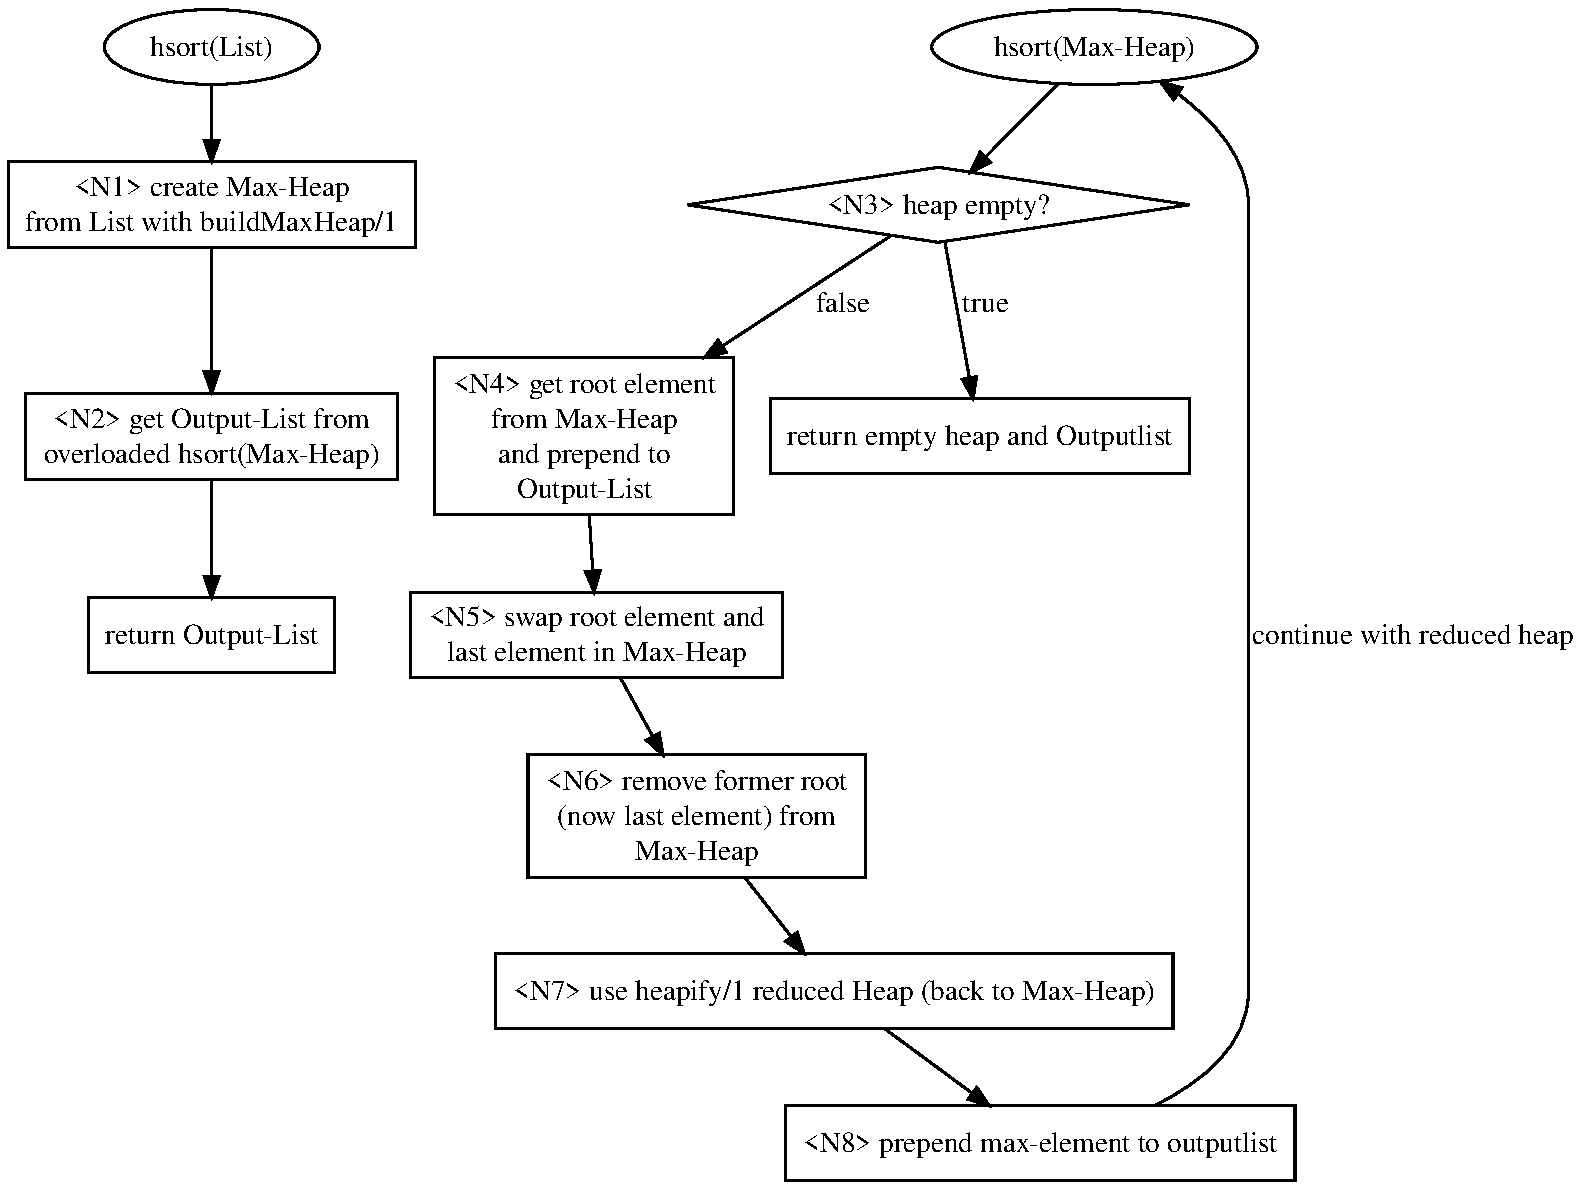
\includegraphics[width = 11cm]{hsort.pdf}\label{fig:hsort}
    \end{figure}

    \begin{figure}[hb]
        \caption{Heapify}
        \centering
        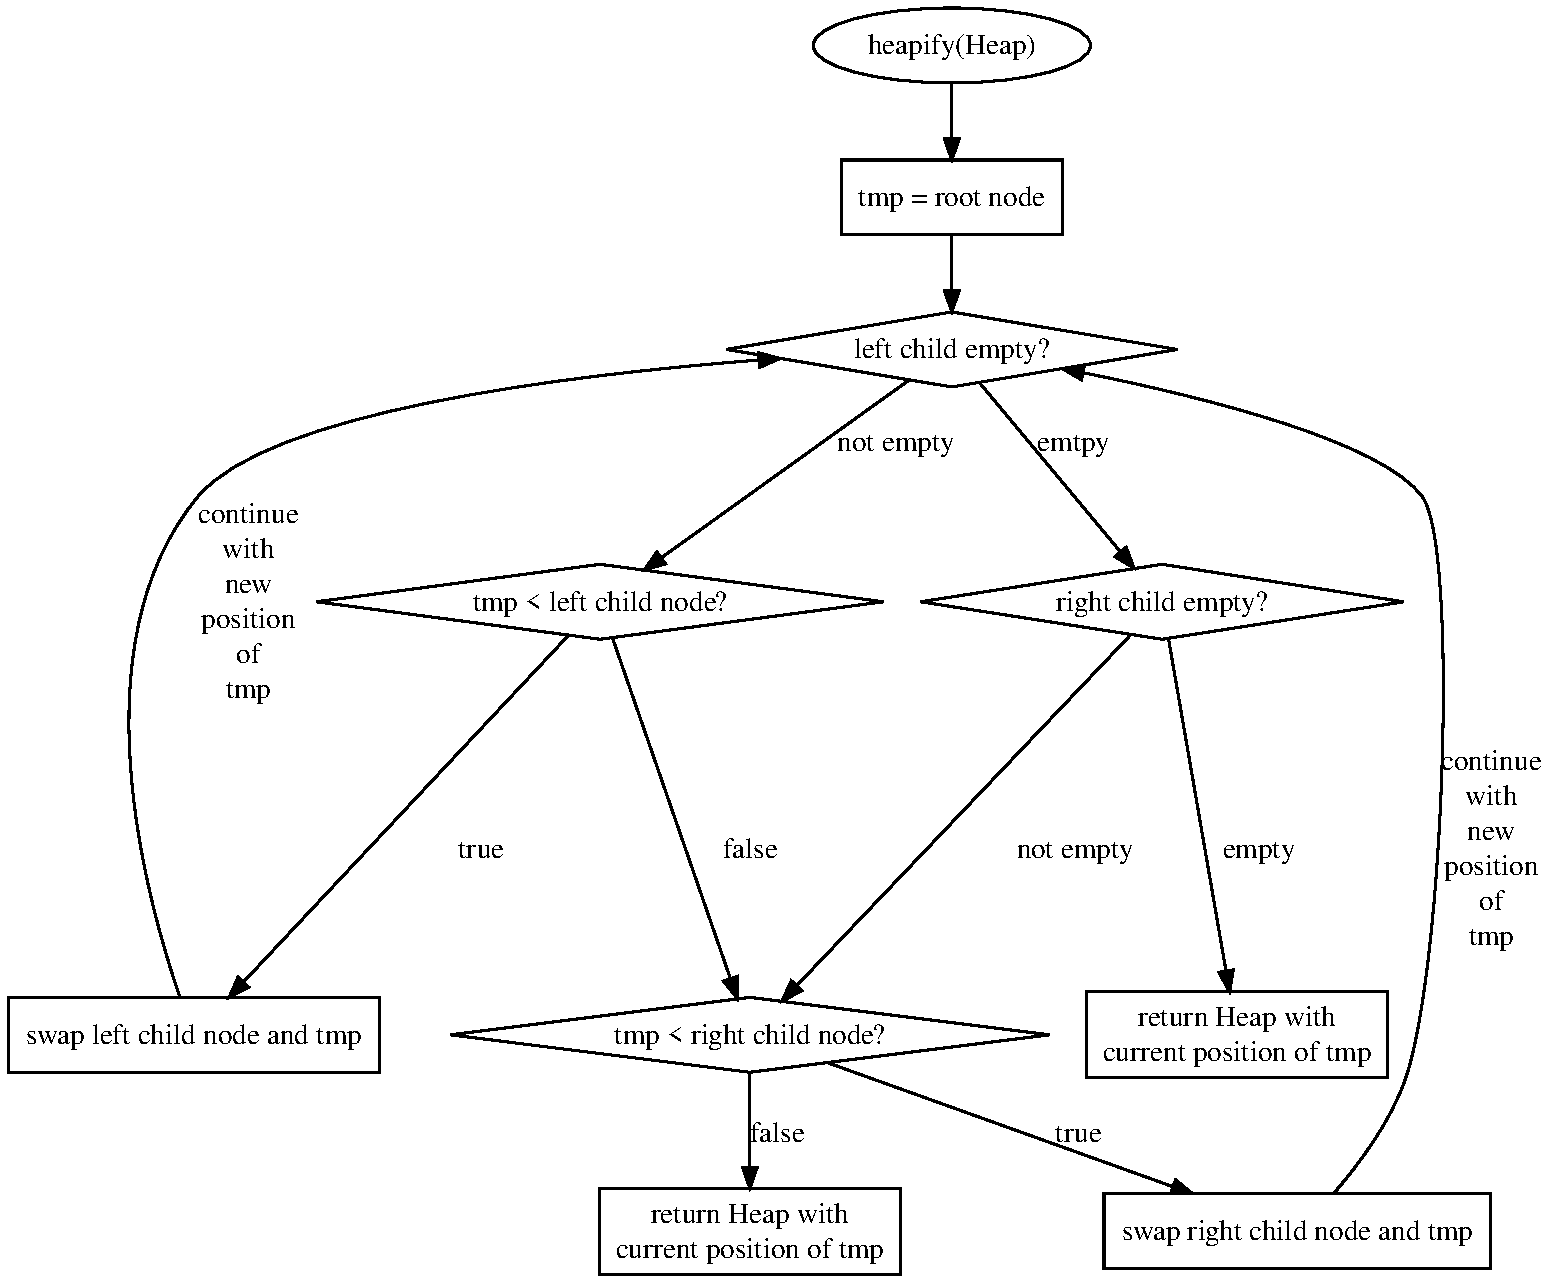
\includegraphics[width = 10cm]{heapify.pdf}\label{fig:heapify}
    \end{figure}

    \begin{figure}[hbt]
        \caption{Build Max-Heap}
        \centering
        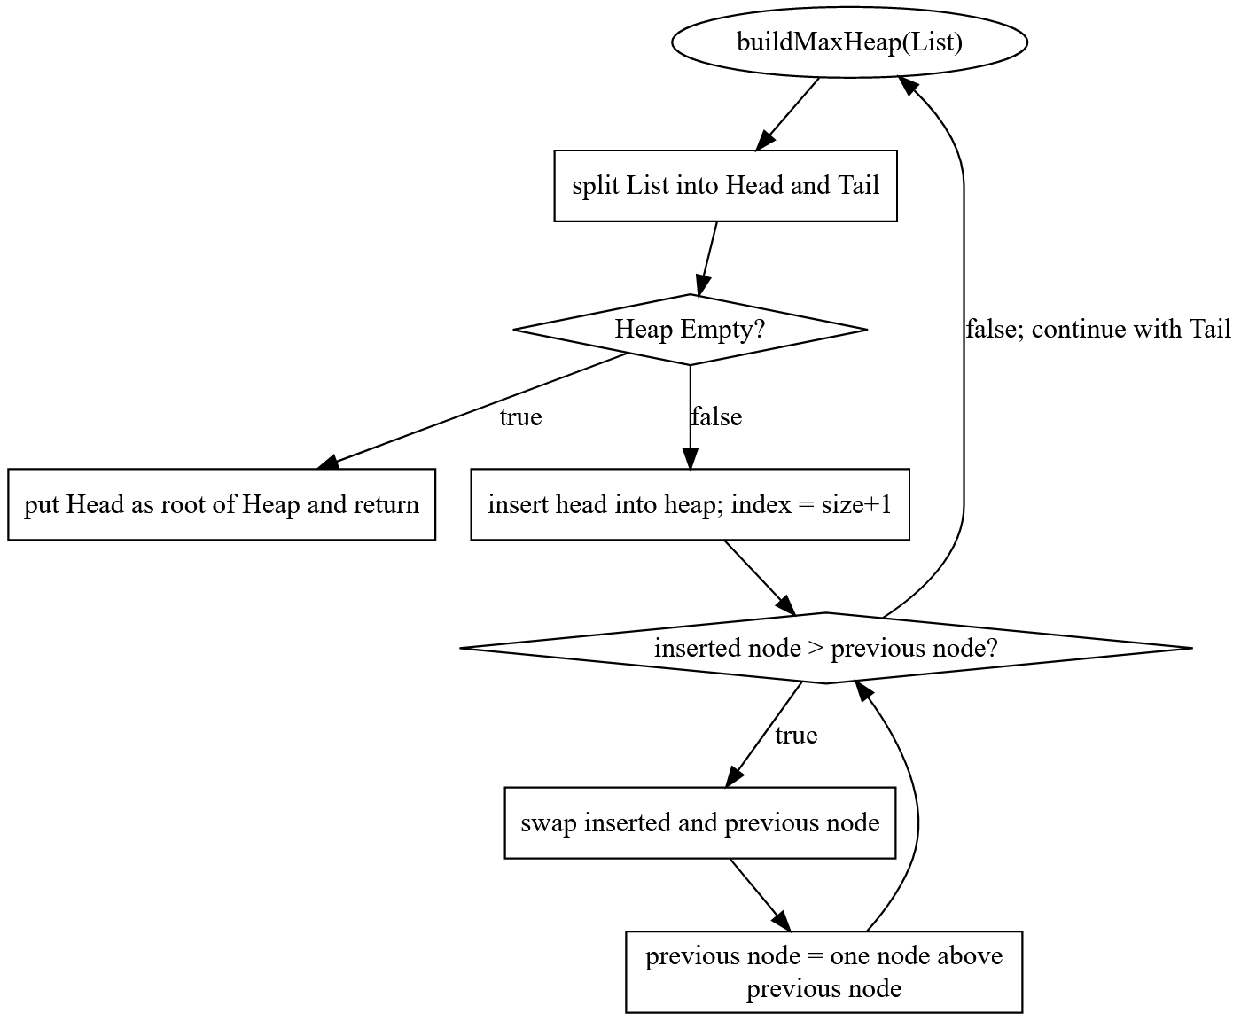
\includegraphics[width = 10cm]{buildMaxHeap.pdf}\label{fig:buildMaxHeap}
    \end{figure}

    \subsection{Laufzeit}\label{subsec:Hlaufzeit}
    Die Laufzeit beträgt im Worst-Case \(O(n\cdot log\ n)\). Dieser tritt
    ein, wenn eine bereits weitgehend vorsortierte Liste vorliegt, da die
    Liste beim Heap-Aufbau gewissermaßen invertiert wird und somit viele
    Vergleiche pro Element erforderlich sind.
    Wünschenswert wäre demnach eine invertiert-sortierte Liste, wodurch die
    Anzahl der Vergleiche auf 1 pro Element minimiert ist.
    Es gilt mit den Laufzeittests herauszufinden, ob unsere
    Komplexitäts--Annahmen realistisch sind.
    Um Heap-Sort hinreichend zu testen, binden wir den Algorithmus erweiternd
    in den Quick-Sort-Test mit ein und stellen beide gegenüber.
    Diese drei Fälle werden untersucht und verglichen:
    \begin{samepage}
        \begin{itemize}
            \item Vorsortierte Liste
            \item Invertiert sortierte Liste
            \item Zufällig generierte Liste
        \end{itemize}
    \end{samepage}


\end{document}
